\documentclass{article}
\usepackage{fontspec}
\usepackage{xcolor}

\usepackage{amsthm}
\usepackage{amsmath}
\usepackage{amssymb}
\usepackage{unicode-math}
\usepackage[makeroom]{cancel}

\usepackage[normalem]{ulem}

\setmainfont{Times New Roman}
\setmathfont{Latin Modern Math}

\setlength\parindent{0em}
\setlength\parskip{0.618em}
\usepackage[a4paper,lmargin=1in,rmargin=1in,tmargin=1in,bmargin=1in]{geometry}

\usepackage{enumitem}

\renewcommand\qed{\blacksquare}

\usepackage{graphicx}

\begin{document}

\begin{center}
  $\mathcal{Dynamical\enskip Systems}$---$\mathcal{Homework}\enskip 6$

  \color{red}R\color{teal}icardo
  \color{red}J\color{cyan}.
  \color{red}A\color{teal}cu$\color{red}{\widetilde{\color{teal}\text{n}}}$\color{teal}a\color{black}

  \color{teal}(\color{red}862079740\color{teal})\color{black}
\end{center}
\vspace{1.618em}



\paragraph{1}

(1)

$\tau = I\alpha,$ and $I = ml^2$, and $\alpha = \frac{d^2\theta}{dt^2}
= \theta^{\prime\prime}$

Let $m = l = g = 1$

$\implies \tau = \theta^{\prime\prime}$

Assume $\tau = -\sin{\theta} -\theta^{\prime}$

$\implies \theta^{\prime\prime} = -\sin{\theta} -\theta^{\prime}$

Which is the second order differential equation for this dampened
system.

(2)

Let $\theta^\prime = \omega$

$\implies \theta^{\prime\prime}= \omega^\prime$

$\implies \omega^\prime = -\sin{\theta} -\theta^{\prime} = -\sin{\theta} -\omega$

So, the non-linear planar system in terms of $(\theta, \omega)$, where
$\omega$ is the angular velocity is as follows:

$(*)
\begin{cases}\theta^\prime = \omega\\ \omega^\prime = -\sin{\theta}
  -\omega\end{cases} $

(3)

Let $\theta^\prime = \omega^\prime = 0$

$\implies \begin{cases} 0 = \omega\\ 0 = -\sin{\theta}\end{cases}
\implies \begin{cases} \omega = 0\\ \theta = k\pi,
  k\in\mathbb{Z}\end{cases} \implies \begin{pmatrix}k\pi\\0\end{pmatrix}$ are the equilibria of $(*)$

$(*) \implies  \begin{pmatrix}\theta^\prime \\
  \omega^\prime\end{pmatrix} = \begin{pmatrix}\omega \\ -\sin{\theta}
  -\omega\end{pmatrix} = \begin{pmatrix}f(\theta, \omega) \\ g(\theta,
  \omega)\end{pmatrix} = \mathcal{F}(\theta,\omega)$

$\implies \text{D}\mathcal{F}(k\pi,0) = \begin{pmatrix} f_{\theta}(k\pi,0) &
  f_{\omega}(k\pi,0)\\ g_{\theta}(k\pi,0)& g_{\omega}(k\pi,0)\end{pmatrix}
= \begin{pmatrix} 0 &
  1 \\ -\cos{k\pi} & -1\end{pmatrix}$

$\implies \text{Tr}(\text{D}\mathcal{F}(k\pi,0)) = -1$ and
$|\text{D}\mathcal{F}(k\pi,0)| = \begin{cases} 1, k$ even$\\-1 , k$ odd$ \end{cases}$

So none of the systems is a center. So, all of the points, are hyperbolic.

Therefore, we can apply \textit{linearization} to all of the points.

p$(\lambda) = \lambda^2 -\text{Tr}(\text{D}\mathcal{F}(k\pi,0))\lambda
+ |\text{D}\mathcal{F}(k\pi,0)|$

p$(\lambda) = 0 \implies \lambda =
\frac{\text{Tr}(\text{D}\mathcal{F}(k\pi,0)) \pm
\sqrt{\text{Tr}(\text{D}\mathcal{F}(k\pi,0))^2 -4|\text{D}\mathcal{F}(k\pi,0)|}}{2}$
\newpage

For $k$ even, $\lambda = \frac{-1 \pm\sqrt{(-1)^2 -4(1)}}{2} =
-\frac{1}{2} \pm\frac{\sqrt{3}}{2}i $

$\implies \underbar{\overline{X}} = e^{-\frac{1}{2}t}\begin{pmatrix}
  \cos(\frac{\sqrt{3}}{2}t) & \sin(\frac{\sqrt{3}}{2}t)\\
  -\sin(\frac{\sqrt{3}}{2}t) &\cos(\frac{\sqrt{3}}{2}t)\end{pmatrix} =
e^{-\frac{t}{2}}R_{-\frac{\sqrt{3}}{2}t}$

It's clear from $(*)$ that it rotates clockwisely, because the
rate of change of the angle is direclty proportional
to the angular velocity---i.e: In QI of the $(\theta,\omega)$-plane,
$\theta^\prime$ is positive. And, $t\rightarrow \infty \implies
e^{-\frac{t}{2}}\rightarrow 0$, so $t\rightarrow \infty \implies $
$\underbar{\overline{X}}\rightarrow 0$.
So $\vec{0}$ is  a spiral sink of $\text{D}\mathcal{F}(k\pi,0)$ when
$k$ is even. By, \textit{linearization}  $\exists
h_1:\mathbb{R}^2\rightarrow \mathbb{R}^2$, a local homomorphism:
$\forall k\in \mathbb{Z}: k$ is even and $ h_1^{-1}(\vec{0}) = \begin{pmatrix}
  k\pi\\0\end{pmatrix}$ is locally a spiral sink of $\mathcal{F}$.

For $k$ odd, $\lambda = \frac{-1 \pm\sqrt{(-1)^2 -4(-1)}}{2} =
-\frac{1}{2} \pm\frac{\sqrt{5}}{2} $

$\implies \lambda_1 = -\frac{1}{2} +\frac{\sqrt{5}}{2}$ and$\lambda_2 =
-\frac{1}{2} -\frac{\sqrt{5}}{2} $

$\text{D}\mathcal{F}(k\pi,0)= \begin{pmatrix} 0 &
    1 \\ 1 & -1\end{pmatrix} $

$(\text{D}\mathcal{F}(k\pi,0) -\lambda_1 I)= \begin{pmatrix} \frac{1}{2} -\frac{\sqrt{5}}{2} &
  1 \\ 1 & -\frac{1}{2} -\frac{\sqrt{5}}{2}\end{pmatrix}\\
=
\begin{pmatrix} \frac{1-\sqrt{5}}{2} &
  1 \\ 1 & -\frac{1+\sqrt{5}}{2}\end{pmatrix}
\rightarrow
\begin{pmatrix} 1 & \frac{2}{1-\sqrt{5}}\frac{1+\sqrt{5}}{1+\sqrt{5}}
 \\ 1 & -\frac{1+\sqrt{5}}{2}\end{pmatrix}
\rightarrow
\begin{pmatrix} 1 & \frac{2(1+\sqrt{5})}{1-5}
 \\ 1 & -\frac{1+\sqrt{5}}{2}\end{pmatrix}
\rightarrow
\begin{pmatrix} 1 & -\frac{1+\sqrt{5}}{2}
  \\ 1 & -\frac{1+\sqrt{5}}{2}\end{pmatrix}
\rightarrow
\begin{pmatrix} 1 & -\frac{1+\sqrt{5}}{2}
 \\ 0 & 0\end{pmatrix}
$

$
\implies v_1 =  \begin{pmatrix}\frac{1+\sqrt{5}}{2}\\1\end{pmatrix}
$


$(\text{D}\mathcal{F}(k\pi,0) -\lambda_2 I)= \begin{pmatrix} \frac{1}{2} +\frac{\sqrt{5}}{2} &
  1 \\ 1 & -\frac{1}{2} +\frac{\sqrt{5}}{2}\end{pmatrix}\\
 \begin{pmatrix} \frac{\sqrt{5}+1}{2} &
  1 \\ 1 & \frac{\sqrt{5} -1}{2}\end{pmatrix}
\rightarrow
\begin{pmatrix} \frac{\sqrt{5}+1}{2} &
  1 \\ \frac{2}{\sqrt{5} -1}\frac{\sqrt{5}+1}{\sqrt{5}+1} & 1\end{pmatrix}
\rightarrow
\begin{pmatrix} \frac{\sqrt{5}+1}{2} &
  1 \\ \frac{2(\sqrt{5}+1)}{5-1} & 1\end{pmatrix}
\rightarrow
\begin{pmatrix} \frac{\sqrt{5}+1}{2} &
  1 \\ \frac{\sqrt{5}+1}{2} & 1\end{pmatrix}
\rightarrow
\begin{pmatrix} \frac{\sqrt{5}+1}{2} &
  1 \\ 0 & 0\end{pmatrix}

$

$
\implies v_2 =  \begin{pmatrix}1 \\ -\frac{1+\sqrt{5}}{2}\end{pmatrix}
$

$\implies x(t)= e^{\lambda_1 t}v_1+e^{\lambda_2 t}v_2$ is the generalized
solution to $\text{D}\mathcal{F}(k\pi,0)$ when $k$ is odd.

$\lambda_1 = -\frac{1}{2} +\frac{\sqrt{5}}{2} \approx 0.6880339887 $ and$\lambda_2 =
-\frac{1}{2} -\frac{\sqrt{5}}{2} \approx -1.6180339887$

$\implies \\
\lim\limits_{t\rightarrow -\infty} x(t) = v_2,\quad$ since
$e^{-\lambda_1\infty} << e^{-\lambda_2\infty}$

and

$\lim\limits_{t\rightarrow \infty} x(t) = v_1,\quad$ since
$e^{\lambda_2\infty} << e^{\lambda_1\infty}$

So, $\vec{0}$ is a saddle of $\text{D}\mathcal{F}(k\pi,0)$, when $k$ is odd, with trajectories coming from the $v_2$ direction
to the $v_1$ direction. By, \textit{linearization} $\exists
h_2:\mathbb{R}^2\rightarrow \mathbb{R}^2$, a local homomorphism:
$\forall k\in \mathbb{Z}: k$ is odd and $ h_2^{-1}(\vec{0}) = \begin{pmatrix}
  k\pi\\ 0\end{pmatrix}$ is locally a saddle of $\mathcal{F}$.

(4)

The dampened pendulum will eventually stop if the angle start's
between strictly between $-\pi$ and $k2pi +\pi$ that's the meaning of
even multiples of $\pi$ being sinks. If, the angular momentum is too big, or too small, that is
outside the bounds outside of the diamonds determined by the saddle points,
then it will get stuck about the odd multiples of $\pi$. The uniqueness part of
the system being nice, won't let the angle increase more that an odd
multiple of $\pi$, and as infinite angular velocity makes no sense,
the only reasonable explanation is that it gets stuck. Actually, what
I think would happen for the low energies is that it gets stuck and
falls, and in the high energies, the string breaks.
\newpage
\paragraph{2}

$(\#)
\begin{cases}
x^\prime = −y\\
y^\prime = x^3 − x.
\end{cases}
$

(1)

$H(x,y) = -\int -y dy + \int x^3-x dx = \frac{1}{2}y^2
+\frac{1}{4}x^4 -\frac{1}{2}x^2 + C$

Let $ C= \frac{1}{4}:
\frac{1}{4}x^4 -\frac{1}{2}x^2 + \frac{1}{4} =
\frac{1}{4}(x^4 -2x^2 + 1) =
\frac{1}{4}(x^2 -1)^2$

$\implies H(x,y) = \frac{1}{2}y^2 +\frac{1}{4}(x^2 -1)^2$

(2)

$X = \{(x, y) \in \mathbb{R}^2 | H(x, y) \leq C\}$ for $0\leq C$

Is $X$ is bounded for each $C$ because the $C$ for each $(x,y)$, the least
upper bound of the set is $C$.

For each $C$, $X = \cup\limits_{c\in [0, C]}
H^{-1}(c)$, the level sets of $H$ for each $c$, where $0 \leq c \leq C$.
Individually each of the level sets are trajectories, since $H$ is hamiltonian. So $X$ is
invariant, as any point in the set will stay in one of the level sets
and $X$ is the union of all those level sets.

In particular, the level sets are curves, so they're closed subsets
of $R^2$, so their union is closed. So, for each $C$, $X$ is a closed and bounded invariant set.

(3)

Letting $x^\prime = y^\prime = 0$ in $(\#)
\implies
\begin{cases}
0= −y\\
0= x^3 − x.
\end{cases}
$

$\implies y = 0$ and $0 = x^3 − x = x(x^2-1) = x(x+1)(x-1) $

$\implies y = 0$ and $(x =0 $ or $ x = 1$ or $x = -1 )$

$\implies \begin{pmatrix}0\\0\end{pmatrix}$ and $\begin{pmatrix}1\\
  0\end{pmatrix}$ and $\begin{pmatrix}-1 \\ 0\end{pmatrix}$ are the
equilibria of $(\#)$


(4)

Consider $\frac{1}{2}y^2 +\frac{1}{4}(x^2 -1)^2 \leq C$

$\implies \frac{1}{2}y^2 \leq C - \frac{1}{4}(x^2 -1)^2$

$\implies y^2 \leq 2C - \frac{1}{2}(x^2 -1)^2 $

$\implies y \leq \pm \sqrt{2C - \frac{1}{2}(x^2 -1)^2}$

Case 0: $C < 0$

Then $C = -D$ some $D > 0$

$\implies y \leq \pm \sqrt{-2D - \frac{1}{2}(x^2 -1)^2}$

$\implies y \leq \pm i\sqrt{2D  +\frac{1}{2}(x^2 -1)^2}$

$y\in \mathbb{R} \implies X = \emptyset$

Case 1: $C = 0$

Reconsider $\frac{1}{2}y^2 +\frac{1}{4}(x^2 -1)^2 \leq 0$

$y^2$ and $(x^2 -1)^2$ are squares, so they're
positive, so a linear combination with positive coefficients is positive. They have no negative
solutions, so the only way their linear combination is equal to $0$ is if they're
both $0$.

So, $y^2 = 0 \implies y=0$

and, $(x^2 -1)^2 = 0 \implies x^2 -1 = 0 \implies x= \pm 1$

So, if $C = 0$, $X$ is the same as two of the equilibrium points we
already had.
\newpage

Case 3: $C = \frac{1}{4}$

Reconsider $\frac{1}{2}y^2 +\frac{1}{4}(x^2 -1)^2 \leq \frac{1}{4}$

$\stackrel{*4}{\implies} 2y^2 +(x^2 -1)^2 \leq 1$

$\stackrel{}{\implies} 2y^2 \leq 1 -(x^2 -1)^2 = 1 -(x^4-2x^2+1) =
-x^4+2x^2 = x^2(2-x^2) = x^2(\sqrt{2} -x)(\sqrt{2} + x)$

$\implies 2y^2\leq x^2 (\sqrt{2} -x)(\sqrt{2} + x)$

For the same reasons, if $x = \pm \sqrt{2}$ or $x=0$, then $y=0$

So, at $\begin{pmatrix}\sqrt{2}\\0\end{pmatrix}$ and
$\begin{pmatrix}0\\0\end{pmatrix}$ and
$\begin{pmatrix}-\sqrt{2}\\0\end{pmatrix}$ the trajectory crosses the
$x$-axis.

Next we consider the function:

$y =  \frac{x\sqrt{(\sqrt{2} -x)(\sqrt{2} + x)}}{\sqrt{2}} = \frac{x\sqrt{2 -x^2}}{\sqrt{2}}$

$y^\prime = (\frac{x\sqrt{2 -x^2}}{\sqrt{2}})^\prime =
\frac{x}{\sqrt{2}}\prime\sqrt{2 -x^2} + \frac{x}{\sqrt{2}}(\sqrt{2 -x^2})^\prime$

$= \frac{1}{\sqrt{2}}\sqrt{2 -x^2} + \frac{x}{\sqrt{2}}
\frac{-2x}{2\sqrt{2 -x^2}}$
$= \frac{1}{\sqrt{2}} (\sqrt{2 -x^2} -\frac{x^2}{\sqrt{2 -x^2}})$

$= \frac{1}{\sqrt{2}}\frac{2 -2x^2}{\sqrt{2 -x^2}}$
$= \frac{1}{\sqrt{2}}^2\frac{2(1 -x^2)}{\sqrt{1 -\frac{x^2}{2}}}$

$= \frac{1 -x^2}{\sqrt{1 -\frac{x^2}{2}}}$

$y^\prime$ is clearly undefined if $x \geq\sqrt{2}$ or $x\leq
\sqrt{2}$. Since $1 -\frac{x^2}{2}< 0$, whenever $x^2 > 2$

For the values of $x$ where $y^\prime$ is defined Let $y^\prime = 0$

$\implies 0 = \frac{1 -x^2}{\sqrt{1 -\frac{x^2}{2}}} \implies 0 = 1 - x^2 \implies x=1 $ or $x= -1$

So $y^\prime$ attains it's bounds at $x=\pm 1$

$y^{\prime\prime} = \left(\frac{1 -x^2}{\sqrt{1 -\frac{x^2}{2}}}\right)^\prime$

$= \frac{(1 -x^2)^\prime\sqrt{1 -\frac{x^2}{2}} -(1 -x^2)\left(\sqrt{1
      -\frac{x^2}{2}}\right)^\prime}{1 -\frac{x^2}{2}}$
$= \frac{-2x\sqrt{1 -\frac{x^2}{2}}
  -(1-x^2)\frac{\frac{-2x}{2}}{2\sqrt{1 -\frac{x^2}{2}}}}{1
  -\frac{x^2}{2}}}$
$= \frac{-2x\sqrt{1 -\frac{x^2}{2}} -(1-x^2)\frac{-x}{2\sqrt{1
      -\frac{x^2}{2}}}}{1 -\frac{x^2}{2}}}$
$= \frac{-2x\sqrt{1 -\frac{x^2}{2}} +\frac{x-x^3}{2\sqrt{1
      -\frac{x^2}{2}}}}{1 -\frac{x^2}{2}}}$
$= \frac{\frac{-4x(1 -\frac{x^2}{2}) +x-x^3}{2\sqrt{1
      -\frac{x^2}{2}}}
}{\frac{2 -x^2}{2}}}$
$= \frac{-4x(1 -\frac{x^2}{2}) +x-x^3}{(2 -x^2)\sqrt{1
      -\frac{x^2}{2}}}$
$= \frac{-4x +2x^3 +x -x^3}{(2 -x^2)\sqrt{1-\frac{x^2}{2}}}$
$= \frac{x(x^2-3)}{(2 -x^2)\sqrt{1 -\frac{x^2}{2}}}$
$= \frac{x(x^2-3)}{(2 -x^2)\frac{1}{\sqrt{2}}\sqrt{2 -x^2}}$
$= \frac{\sqrt{2}\enskip x(x^2-3)}{(2 -x^2)^\frac{3}{2}}$

By the second derivative test:


$y^{\prime\prime}(-1) = \frac{\sqrt{2}\enskip -1((-1)^2-3)}{(2
  -(-1)^2)^\frac{3}{2}} = 2\sqrt{2} >  0 \implies x = -1$ is a local
minimum of $y$

$\implies x = -1$ is a local maximum of $-y$

$y^{\prime\prime}(1) = \frac{\sqrt{2}\enskip 1(1^2-3)}{(2
  -1^2)^\frac{3}{2}} = -2\sqrt{2} <  0 \implies x = 1$ is a local
maximum of $y$

$\implies x = 1$ is a local minimum of $-y$

So $H^{-1}(\frac{1}{4})$ has 3 orbits, because $C = \frac{1}{4}$ is
the only orbit that includes the equilibrium point
$\begin{pmatrix}0\\0\end{pmatrix}$. That's the homoclinic point. And
there are two homoclinic orbits, one to the right through $x = 1$, and
one through the left through $x = -1$.

The direction is counterclockwise,
since $(\#) \implies x^\prime = -y$, and on QI of the $(x,y)-$plane,
$y$ is posititive, so $x$ is decreasing and on QIV $y$ is negative so,
$x$ is increasing.
\newpage
Case 2: $0<C<\frac{1}{4}$

Consider, $2y^2 < x^2 (\sqrt{2} -x)(\sqrt{2} + x)$, we have 2
cycles for each $C$ because it is the area inside the homoclinic
orbits of case 3. And it doesn't contract to a point because that's
case 1. So, each of the left loops will cross the $x-$axis on points
greater than $-\sqrt{2}$ and smaller than $0$. Similarly for the right
loops, they'll cross the $x-$axis on points greater than $0$ and
smaller than $\sqrt{2}$.

The $y-$bounds of each loop will be between the bounds
of our $y$ function. So, reconsidering $y$ of case 3:

$y(-1) =
\frac{-1\sqrt{2 -(-1)^2}}{\sqrt{2}} = -\frac{1}{\sqrt{2}} $
 and
$y(1) =  \frac{1\sqrt{2 -1^2}}{\sqrt{2}} = \frac{1}{\sqrt{2}} $

So, the loops will be between $-\frac{1}{\sqrt{2}}$ and
$\frac{1}{\sqrt{2}}$.

Case 4: $\frac{1}{4} < C$

Consider, $2y^2 > x^2 (\sqrt{2} -x)(\sqrt{2} + x)$, we have 1
cycle for each $C$ because it is the area outside the homoclinic
orbits of case 3. So, the loops will cross the $x-$axis on points
smaller than $-\sqrt{2}$ and greater than $\sqrt{2}$.

So, the loops will be between values of $-\frac{1}{\sqrt{2}} -\varepsilon$ and
$\frac{1}{\sqrt{2}} + \varepsilon$, some $\varepsilon>0$.

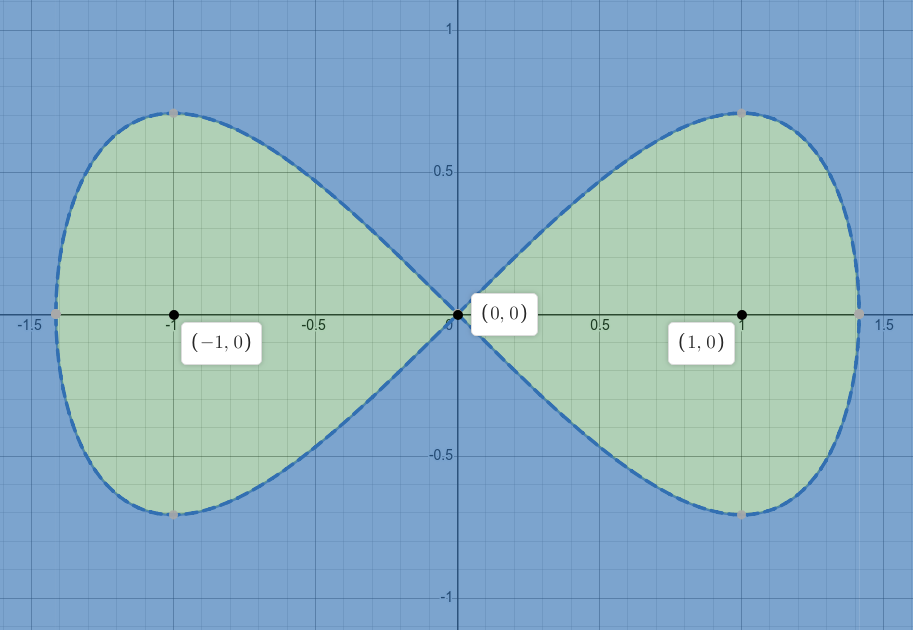
\includegraphics[width=\textwidth]{2}

\end{document}
%%% Local Variables:
%%% mode: latex
%%% TeX-master: t
%%% End:
